\documentclass[a4paper,14pt]{extarticle} % the default "article" class is limited to 12pt, but you can go up to 14, 17 or 20 points if you use the "extarticle" class
\usepackage{cmap} % make LaTeX PDF output copy-and-pasteable
\usepackage[T2A]{fontenc}
\usepackage[utf8]{inputenc}
\usepackage[english,ukrainian]{babel}

\usepackage{amssymb, amsfonts, mathtools, amsmath, enumerate}
\usepackage{indentfirst} % set an additional space before a paragraph at the begining of a new section
\usepackage{setspace}
\usepackage{textcomp}

\usepackage{dsfont} % indicator symbol
\usepackage{leftidx} % this package enables left subscripts and superscripts in math mode

\usepackage{import} % for adding a file by path https://tex.stackexchange.com/questions/246/when-should-i-use-input-vs-include

\usepackage{geometry} 
\geometry{left=1.25cm}
\geometry{right=1.25cm}
\geometry{top=1cm}
\geometry{bottom=2cm}

\setlength{\arrayrulewidth}{0.3mm} % this sets the thickness of the borders of the table
\setlength{\tabcolsep}{12pt} % the space between the text and the left/right border of its containing cell is set to 18pt with this command
\renewcommand{\arraystretch}{1.5} % the height of each row is set to 1.5 relative to its default height

\usepackage[table,xcdraw,dvipsnames]{xcolor}
\usepackage{multirow}
\usepackage{color}
% 1) tutorial about xcolor:  https://www.overleaf.com/learn/latex/Using_colours_in_LaTeX
% 2) huge tutorial about xcolor: https://latex-tutorial.com/color-latex/ 
% 3) RGB calculator: https://www.w3schools.com/colors/colors_rgb.asp

\usepackage{hyperref}
\definecolor{linkcolor}{HTML}{0000FF}
\definecolor{urlcolor}{HTML}{0000FF} 
\hypersetup{pdfstartview=FitH, unicode=true, linkcolor=linkcolor, urlcolor=urlcolor, colorlinks=true}

\usepackage{graphicx}
\usepackage{wrapfig}
\usepackage{float}

\parskip=1mm % space between paragraphs

% enumerating equations according to the section number 
% plus resetting each numeration inside each section
\numberwithin{equation}{section}

% numbering only sections in the table of contents (the "1" nesting level)
% thus numbering equations only according to the section number
\setcounter{secnumdepth}{1}

\usepackage{listingsutf8} % origin: \usepackage{listings}

\lstset{
    frame=single,
    language=Python,
    aboveskip=3mm,
    belowskip=3mm,
    columns=flexible,
    basicstyle=\small\ttfamily,
    numbers=left,
    numberstyle=\tiny\color{gray},
    commentstyle=\color{OliveGreen},
    stringstyle=\color{Mahogany},
    morestring=[b]''',
    showstringspaces=false,
    keywordstyle=\bfseries\color{blue},
    emph={[1]import, as, for, while, return}, emphstyle={[1]\bfseries\color{Mulberry}},
    emph={[2]range}, emphstyle={[2]\bfseries\color{brown}},
    breaklines=true,
    breakatwhitespace=true,
    tabsize=4,
    extendedchars=false, % to use ukrainian text in a code
    inputencoding=utf8 % to use ukrainian text in a code
}

\begin{document}

\import{Title/}{title}

\section*{Завдання 1}

\textit{Змоделювати ланцюг Маркова із заданою матрицею перехідних імовірностей:}
\begin{equation*}
    P = 
    \begin{pmatrix}
        0.5 & 0.5 & 0.0 & 0.0 & 0.0 & 0.0 \\
        0.5 & 0.0 & 0.5 & 0.0 & 0.0 & 0.0 \\
        0.0 & 0.0 & 0.5 & 0.3 & 0.2 & 0.0 \\
        0.0 & 0.0 & 0.3 & 0.0 & 0.0 & 0.7 \\
        0.0 & 0.0 & 0.2 & 0.0 & 0.8 & 0.0 \\
        0.0 & 0.0 & 0.0 & 0.7 & 0.0 & 0.3 \\
    \end{pmatrix}
\end{equation*}

З вигляду матриці перехідних імовірностей робимо висновок, що ланцюг Маркова складається з шести станів. Тож, наприклад, покладемо множину станів таким чином: $E=\{1,2,3,4,5,6\}$. Наступним кроком на основі матриці $P=(p_{ij})_{i,j\in E}$ введемо допоміжні інтервали $D_{ij}$ так, щоб 
\begin{align*} 
    &\forall i,j\in E: |D_{ij}| = p_{ij} \\ 
    &\forall i\in E: \sum\limits_{j\in E}D_{ij}=1
\end{align*} 

Крім того, покладемо функцію $\psi: E\times[0,1] \rightarrow E$ так:
\[ \psi(i,u)=\sum\limits_{j\in E}\mathds{1}(u\in D_{ij})\cdot j \]

Тоді, задаючи першу ланку ланцюга рівномірно над множиною станів $E$, основний ітераційний алгоритм генерування усіх наступних елементів ланцюга Маркова матиме вид:

\begin{lstlisting}[firstnumber=1, label = code: task 1, caption = Генерування ланцюга Маркова]
    x0 = random.randint(0,E[-1])
    x.append(x0)
    
    for i in range(N):
        u = random.uniform(0,1)
        offer = psi(u,x[-1])
        x.append(offer)
\end{lstlisting}

\vspace{0.4cm}
Тож виконаємо моделювання достатньо великого за довжиною ланцюга з параметром $N=5000$. Обчисливши частоту відвідин ланцюгом кожного з шести станів, матимемо наближення інваріантного розподілу:
\[ \pi=(0.0,\ 0.0,\ 0.2434,\ 0.2446,\ 0.2648,\ 0.2474) \] 

В той час як справжній інваріантний розподіл $\pi^*$, який знаходиться як розв'язок рівняння $\pi^*P=\pi^*$, має вид:
\[ \pi^*=(0.0,\ 0.0,\ 0.25,\ 0.25,\ 0.25,\ 0.25) \] 

Обчислимо середню абсолютну похибку між отриманим наближенням $\pi$ та розподілом $\pi^*:$ 
\[ \delta_{\text{\tiny MAE}}(\pi,\pi^*)=\frac{1}{|E|}\sum\limits_{i\in E}|\pi_{i}-\pi^*_{i}|= 0.00489 \]

Зауважуємо, що значення похибки є малим, що свідчить про достатньо високу ефективність алгоритму МСМС. Наостанок проведемо генерування ланцюга Маркова для, напркилад, таких значень довжин ланцюга:
\[ N=100,200,300,\ldots,99\;800,99\;900,10\;000 \]

При цьому щоразу генеруватимемо ланцюг, починаючи з іншого початкового стану, який обиратимемо рівномірно на множині $E$. На графіку нижче показані значення середньої абсолютної похибки в залежності від величини $N:$

\begin{figure}[H]
    \center{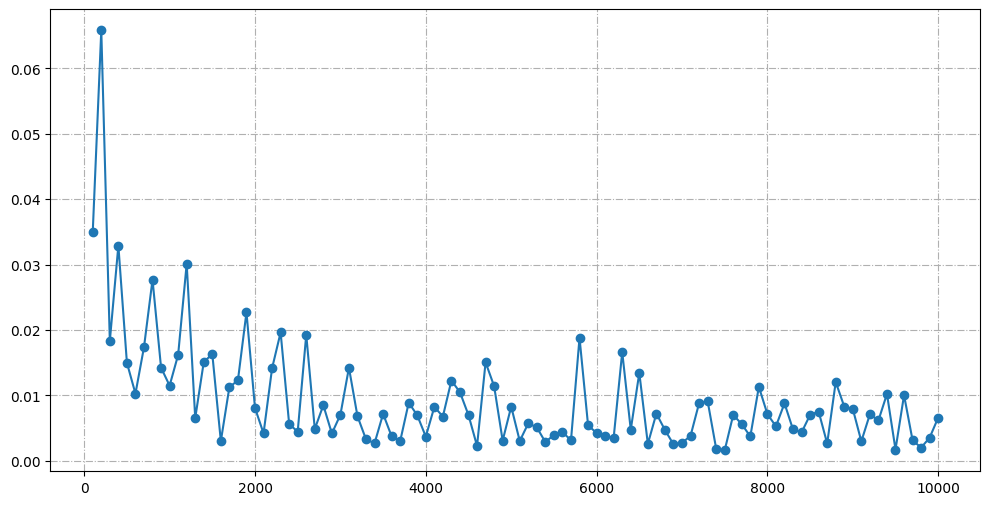
\includegraphics[width=1\linewidth]{images/task 1.png}}
    \caption{Значення $\delta_{\text{\tiny MAE}}(\pi,\pi^*)$ (вісь ординат) в залежності від $N$ (вісь абсцис)}
    \label{figure: task 1}
\end{figure}

Бачимо, що вже при перевищенні межі в $N=2000$ станів досягається достатньо висока точність відповідності між інваріантними розподілами згенерованого та <<оригінального>> ланцюгів. 

\newpage
\section*{Завдання 2}

\textit{Змоделювати ланцюг Маркова, для якого розподіл Зіффа з параметром $a=4$ є інваріантним.} \\

Схематично генерування ланцюга Маркова відрізнятиметься від попереднього завдання тим, що цього разу функція $\psi(i,u)$ обчислюватиметься за допоміжними інтервалами деякої симетричної матриці $Q$, яка є наближенням (або припущенням щодо) матриці перехідних імовірностей. Наприклад, покладемо матрицю $Q$ такою, яка відповідає випадковому блуканню на множині станів $E=\{1,2,3,\ldots,M\}$, де візьмемо $M=50:$
\begin{equation*}
    Q = 
    \begin{pmatrix}
        0.5 & 0.5 & 0.0 & \ldots & 0.0 & 0.0 & 0.0 \\
        0.5 & 0.0 & 0.5 & \ldots & 0.0 & 0.0 & 0.0 \\
        0.0 & 0.5 & 0.0 & \ldots & 0.0 & 0.0 & 0.0 \\
        & \vdots & & \vdots & & \vdots & \\
        0.0 & 0.0 & 0.0 & \ldots & 0.0 & 0.5 & 0.0 \\
        0.0 & 0.0 & 0.0 & \ldots & 0.5 & 0.0 & 0.5 \\
        0.0 & 0.0 & 0.0 & \ldots & 0.0 & 0.5 & 0.5 \\
    \end{pmatrix}
\end{equation*}

Крім того, приймання/відхилення для стану $i$ чергової пропозиції нового стану $j$ залежатиме від величин $\alpha_{ij}:$
\[ \alpha_{ij}=\min\left\{\frac{i^a}{j^a},\ 1\right\} \] 

Таким чином, задаючи перший стан ланцюга рівномірно над множиною станів $E$, основний ітераційний алгоритм генерування усіх наступних $N=800$ елементів ланцюга Маркова матиме вид:

\begin{lstlisting}[firstnumber=1, label = code: task 2, caption = Генерування ланцюга Маркова]
    x0 = random.randint(0,M-1)
    x.append(x0)
    
    for i in range(N):
        u = random.uniform(0,1)
        offer = psi(u,x[-1])
    
        alpha = min(pow(x[-1],a)/pow(offer,a), 1)
    
        v = random.uniform(0,1)
        if v <= alpha:
            x.append(offer)
        else:
            x.append(x[-1])
\end{lstlisting}

Отримавши згенерований ланцюг, порівняємо гістограму отриманого розподілу та гістограму вибірки з розподілу Зіффа (згенерованої вбудованими методами мови \texttt{Python}). Бачимо, що графіки мають високу схожіть:

\begin{figure}[H]
    \begin{minipage}[H]{0.49\linewidth}
        \center{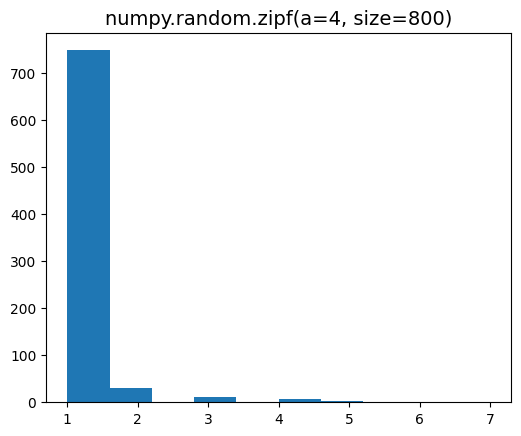
\includegraphics[width=1\linewidth]{images/task 2.1.png}} 
        а) Генерація вбудованими методами мови \texttt{Python}
    \end{minipage}
    \hfill
    \begin{minipage}[H]{0.49\linewidth}
        \center{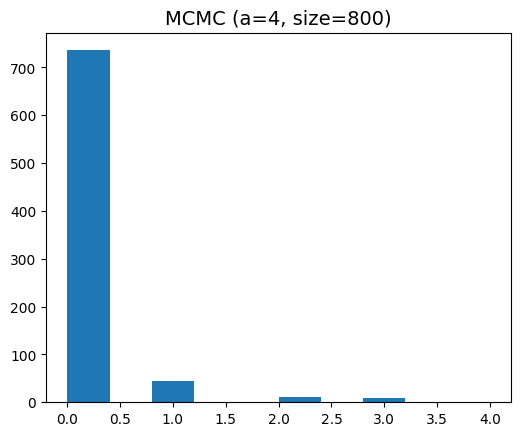
\includegraphics[width=1\linewidth]{images/task 2.2.png}} 
        б) Генерація методами згідно умов Завдання 2
    \end{minipage}
\end{figure}

\newpage
\section*{Завдання 3}

\textit{Змоделювати Бета-розподіл з параметрами $a=2$ та $b=5$ за допомогою алгоритму Метрополіса - Гастінга.} \\

У цьому завданні генерування ланцюга Маркова зводитиметься виключно до роботи з величинами $\alpha_{xx'}$. Наприклад, для поточного стану $x$ прийняття чи відхилення нової пропозиції $x'$ спиратиметься на коефіцієнти виду: \\

\[ \alpha_{xx'}=\min\left\{\frac{{x'}^a(1-{x'})^{b-1}}{x^a(1-x)^{b-1}},\ 1\right\} \] \\

Отже, задаючи перший стан ланцюга $X_0\sim u(0,1)$ рівномірно на відрізку $[0,1]$, основний ітераційний алгоритм генерування усіх наступних $N=1000$ елементів ланцюга Маркова матиме вид: \\

\begin{lstlisting}[firstnumber=1, label = code: task 3, caption = Генерування ланцюга Маркова]
    x0 = random.uniform(0,1)
    x.append(x0)
    
    for i in range(N):
        offer = random.uniform(0,1)
    
        numerator = pow(offer,a-1)*pow((1-offer),b-1)
        denominator = pow(x[-1],a-1)*pow((1-x[-1]),b-1)
        alpha = min(numerator/denominator, 1)
    
        v = random.uniform(0,1)
        if v <= alpha:
            x.append(offer)
        else:
            x.append(x[-1])
\end{lstlisting}

\vspace{0.4cm}
Згенерувавши ланцюг, порівняємо гістограму отриманого розподілу та гістограму вибірки з Бета-розподілу (згенерованої вбудованими методами мови \texttt{Python}). Бачимо, що графіки, знову ж таки, дуже подібні (порівняльні графіки зображені на наступній сторінці).

\begin{figure}[H]
    \begin{minipage}[H]{0.49\linewidth}
        \center{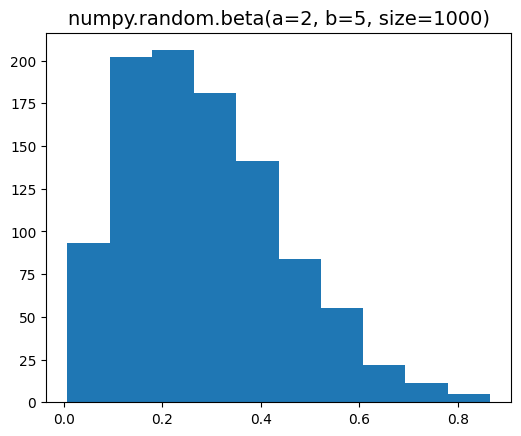
\includegraphics[width=1\linewidth]{images/task 3.1.png}} 
        а) Генерація вбудованими методами мови \texttt{Python}
    \end{minipage}
    \hfill
    \begin{minipage}[H]{0.49\linewidth}
        \center{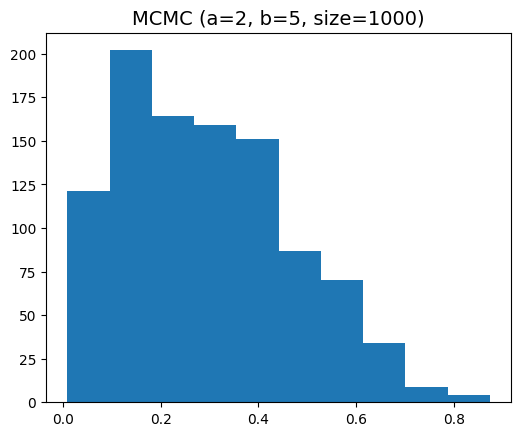
\includegraphics[width=1\linewidth]{images/task 3.2.png}} 
        б) Генерація методами згідно умов Завдання 3
    \end{minipage}
\end{figure}

\newpage
\section*{Завдання 4}

\textit{Побудувати байесову оцінку за допомогою алгоритму МСМС.} \\

Нехай задано розподіл виду:
\[ f_{\Theta|Y}(\theta|y)\sim e^{-\frac{1}{2\sigma^2}(y-\theta)^2} \cdot e^{-\frac{1}{2\sigma^2}(\theta-\mu)^2}, \]

де параметри $y=3,\ \mu=0,\ \sigma^2=1$. Маємо на меті згенерувати такий ланцюг Маркова, для якого цей розподіл є інваріантним, при чому прийняття/відхилення для стану $x$ чергової пропозиції $x'$ відбуватиметься в результаті аналізу значень таких величин:
\[ \alpha_{xx'}=\min\left\{\frac{f_{\Theta|Y}(x'\;|\;y)}{f_{\Theta|Y}(x\;|\;y)},\ 1\right\} \] 

Задаючи перший стан ланцюга $X_0\sim N(\mu,\tau^2)$, основний ітераційний алгоритм генерування усіх наступних $N=10\;000$ елементів ланцюга Маркова (при заданих значеннях $\tau^2=4,\ d=1$) матиме вид:

\begin{lstlisting}[firstnumber=1, label = code: task 4, caption = Генерування ланцюга Маркова]
    x0 = np.random.normal(mu,tau**2)
    x.append(x0)

    for i in range(N):
        offer = x[-1] + np.random.normal(mu,d**2)

        numerator = np.exp(-pow(y-offer,2)/(2*sigma**2)) * np.exp(-pow(offer-mu,2)/(2*sigma**2))
        denominator = np.exp(-pow(y-x[-1],2)/(2*sigma**2)) * np.exp(-pow(x[-1]-mu,2)/(2*sigma**2))
        alpha = min(numerator/denominator, 1)

        v = random.uniform(0,1)
        if v <= alpha:
            x.append(offer)
        else:
            x.append(x[-1])
\end{lstlisting}

\vspace{0.4cm}

При цьому, теоретичне математичне сподівання та дисперсія заданого розподілу матимуть значення:
\[ M(\theta|Y=y)=2.4, \ D(\theta|Y=y)=0.8 \]

Спробуємо порівняти щойно наведені показники з характеристиками згенерованого в результаті алгоритму МСМС ланцюга Маркова. Зобразимо на наступній сторінці гістограму елементів змодельованого ланцюга (Рис. \ref{figure: task 4.1}). 

\begin{figure}[H]
    \center{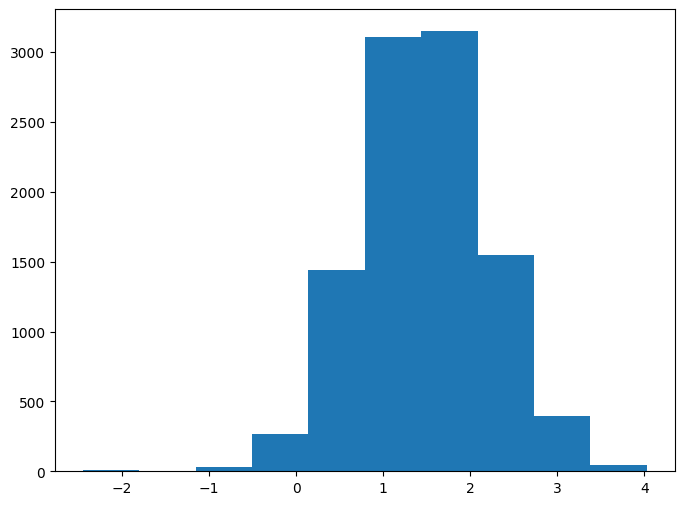
\includegraphics[width=0.8\linewidth]{images/task 4.1.png}}
    \caption{Гістограма утвореного ланцюга Маркова}
    \label{figure: task 4.1}
\end{figure}

Вибіркове середнє та вибіркова дисперсія в даному випадку дорівнюють: \\

\[ \overline{X}=1.4665, \ S^2=0.5318 \] \\

Наостанок прослідкуємо за елементами $X_n$ від ітерації до ітерації при різних значеннях параметра $d:$ \\

\[ d_1=100,\ d_2=1,\ d_3=0.1 \] \\

З графіку, наведеному на наступній сторінці (Рис. \ref{figure: task 4.2}), можна помітити, що при значенні параметра $d_1=100$ елементи змінюються <<надзвичайно грубими сходинками>>. При $d_2=1$ <<сходинки>> є доволі дрібними (особливо в порівнянні з попереднім випадком). Водночас при значенні $d_3=100$ згенеровані елементи ланцюга змінюються дуже динамічно, так що <<сходинки>> майже не проглядаються.

Зауважимо, що для наочності відмінностей між згенерованими ланцюгами, графіки, які відповідають значенням параметрів $d_2$ та $d_3$ продемонстровані лише на перших $500$ елементах ланцюга (однак вибіркові середні та дисперсія обчислені на усьому масиві з $N=10\;000$ ланок).

\begin{figure}[H]
    \center{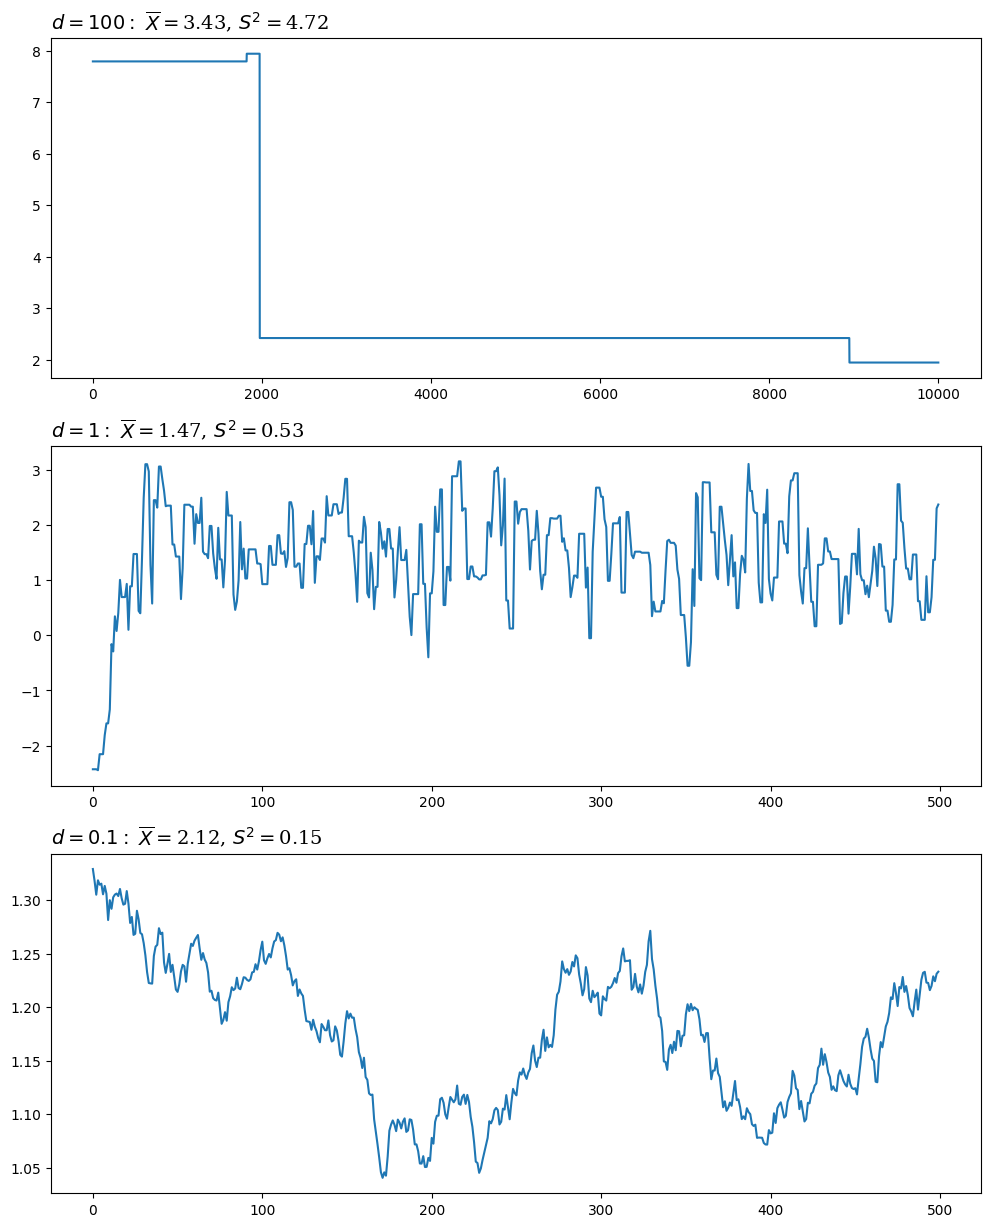
\includegraphics[width=1\linewidth]{images/task 4.2.png}}
    \caption{Значення елементів ланцюга від ітерації до ітерації}
    \label{figure: task 4.2}
\end{figure}

\newpage
\section*{Завдання 5}

\textit{Оцінити кількість k-розфарбовок графа, що складається з $10$ вершин, при кольорах $k=3$ та $k=4$ як кількість різних станів, спостережених за $N=10\;000$ ітерацій.} \\

Спершу розглянемо випадок k-розмальовок графа над такими трьома кольорами: $\{\text{<<green>>, <<blue>>, <<yellow>>}\}$. Отже, нехай початковим станом ланцюга Маркова задана така 3-розмальовка з десяти вершин:

% trim={<left> <lower> <right> <upper>}
\begin{figure}[H]
    \center{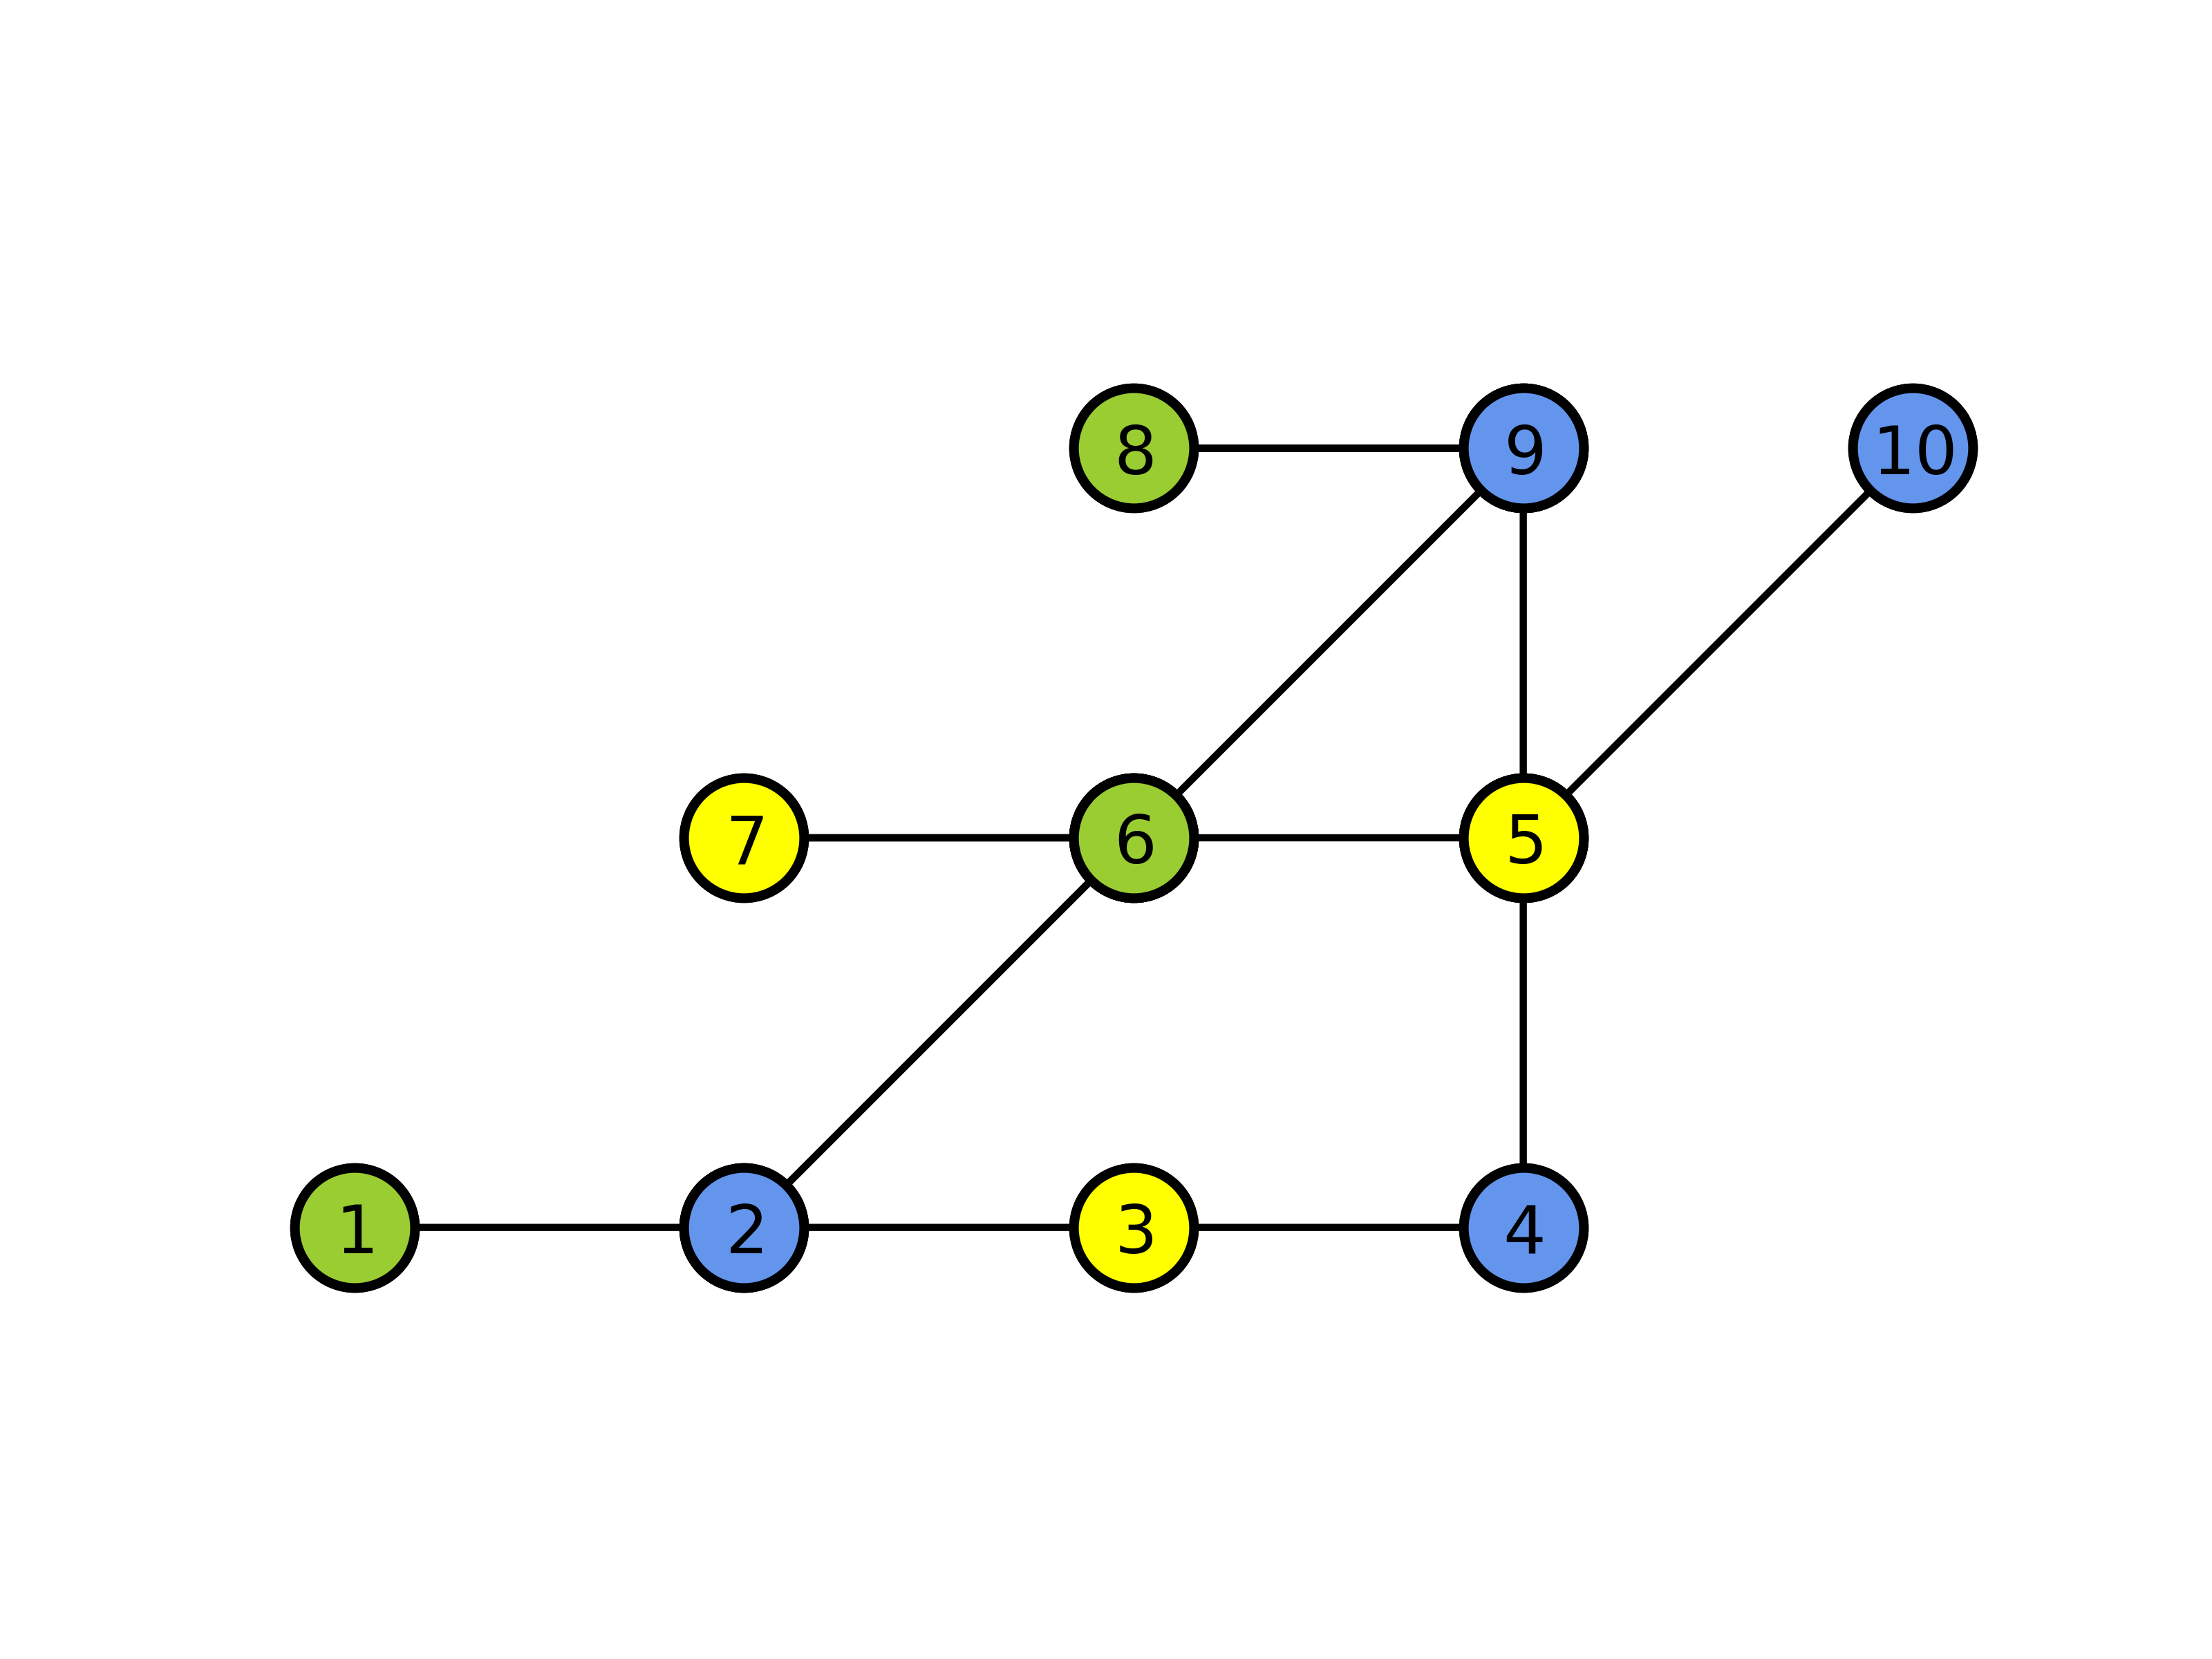
\includegraphics[trim={1.5cm 1.5cm 1.5cm 1.5cm}, clip, width=0.8\linewidth]{images/task 5.1.png}}
    \caption{Початковий стан ланцюга 3-розмальовок}
    \label{figure: task 5.1}
\end{figure}

При цьому основне правило розташування кольорів у графі полягає в тому, що ніякі дві сполучені ребром вершини не мають мати однаковий колір. Побудуємо на множині всіх 3-розфарбовок графа такий ланцюг Маркова, щоб його інваріантний розподіл збігався з рівномірним розподілом на цій множині.

Тож нехай задана деяка початкова розфарбовка (Рис. \ref{figure: task 5.1}). Алгоритм генерування наступних ланок ланцюга Маркова полягатиме у рівномірному виборі однієї з вершин графа та подальшому рівномірному виборі для обраної вершини з множини її допустимих кольорів (при фіксованих кольорах інших вершин) деякого нового кольору (включаючи можливий вибір того самого кольору, який наразі має вершина).

Продемонструємо моделювання такого ланцюга для, наприклад, $N=9$ ланок. На графіку нижче біля кожної 3-розфарбовки позначений її порядковий номер (тобто номер ітерації алгоритму) та індекс поточного стану (початкову ланку на Рис.~\ref{figure: task 5.1} позначимо станом 0).

\begin{figure}[H]
    \center{\includegraphics[trim={4cm 4cm 4cm 4cm}, clip, width=1\linewidth]{images/task 5.2.png}}
    \caption{Графік $N=9$ ітерацій алгоритму МСМС}
    \label{figure: task 5.2}
\end{figure}

Таким чином, якщо протягом алгоритму чергова розфарбовка є новою для згенерованого ланцюга, то їй присвоюється новий унікальний порядковий індекс стану. Якщо ж утворений граф повторює якусь вже наявну розфарбовку, йому присвоєються такий індекс стану, який відповідає повтореній розфарбовці.

Виконавши $N=10\;000$ ітерацій алгоритму генерування ланцюга Маркова, побудуємо гістограму послідовності станів (бачимо, що усього налічується 128 різних 3-розфарбовок): 

\begin{figure}[H]
    \center{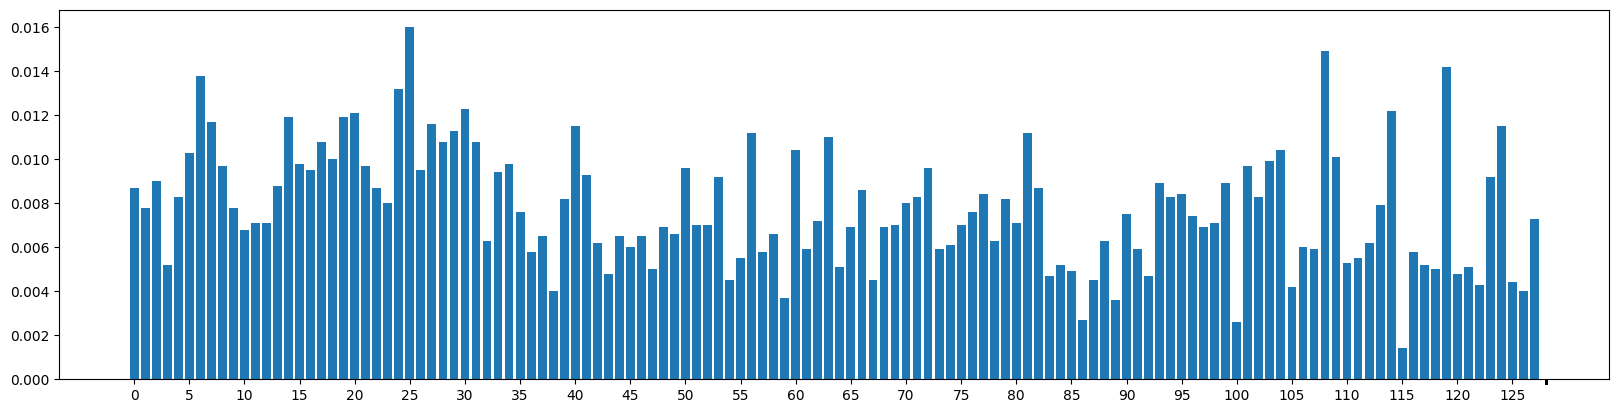
\includegraphics[width=1\linewidth]{images/task 5.3.png}}
    \caption{Гістограма станів 3-розфарбовок}
    \label{figure: task 5.3}
\end{figure}

\newpage

Аналогічним чином розглянемо випадок k-розмальовки графа над чотирма кольорами: $\{\text{<<green>>, <<blue>>, <<yellow>>, <<red>>}\}$. Нехай початковим станом ланцюга Маркова задана така 4-розмальовка з десяти вершин:

% trim={<left> <lower> <right> <upper>}
\begin{figure}[H]
    \center{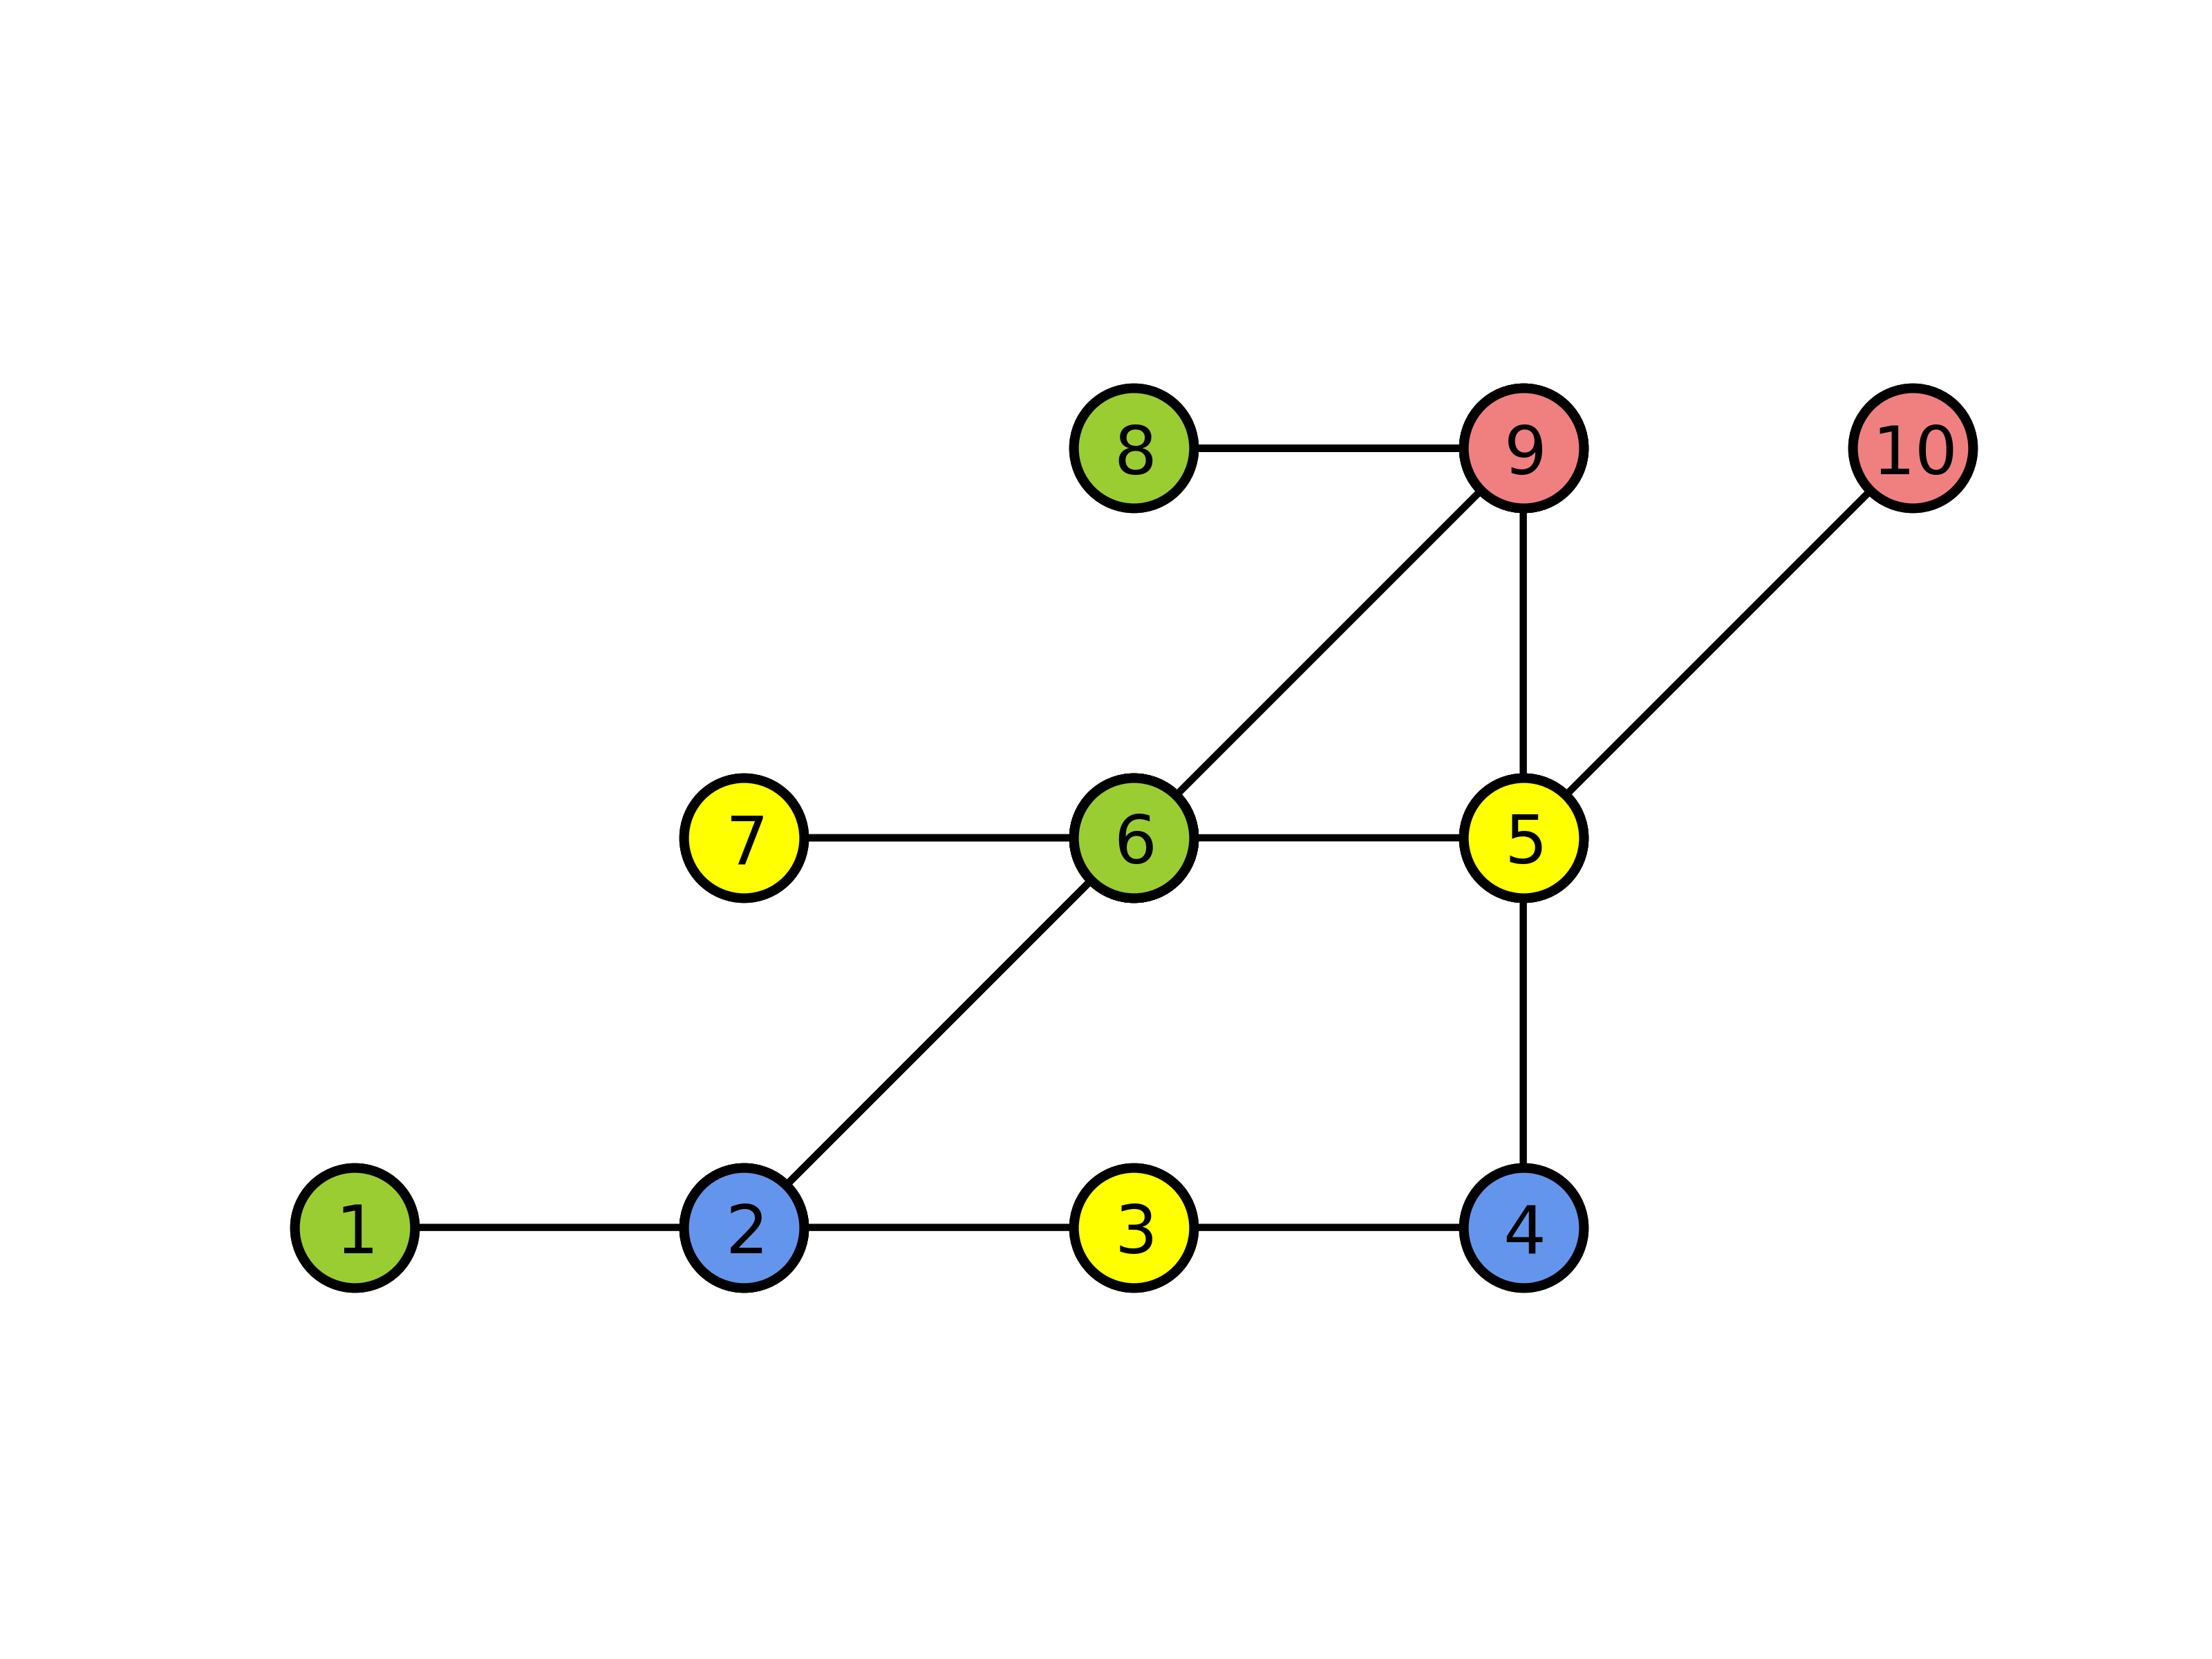
\includegraphics[trim={1.5cm 1.5cm 1.5cm 1.5cm}, clip, width=0.8\linewidth]{images/task 5.4.png}}
    \caption{Початковий стан ланцюга 4-розмальовок}
    \label{figure: task 5.4}
\end{figure}

Задля наочності знову продемонструємо моделювання такого ланцюга для, наприклад, $N=9$ ланок. На графіку (Рис. \ref{figure: task 5.5}) біля кожної 4-розфарбовки позначений її порядковий номер (тобто номер ітерації алгоритму) та індекс поточного стану (при цьому початкову ланку на Рис.~\ref{figure: task 5.4} позначимо станом 0).

Виконавши $N=10\;000$ ітерацій алгоритму генерування ланцюга Маркова, побудуємо гістограму послідовності станів. Як висновок бачимо, що усього налічується 145 різних 4-розфарбовок: 

\begin{figure}[H]
    \center{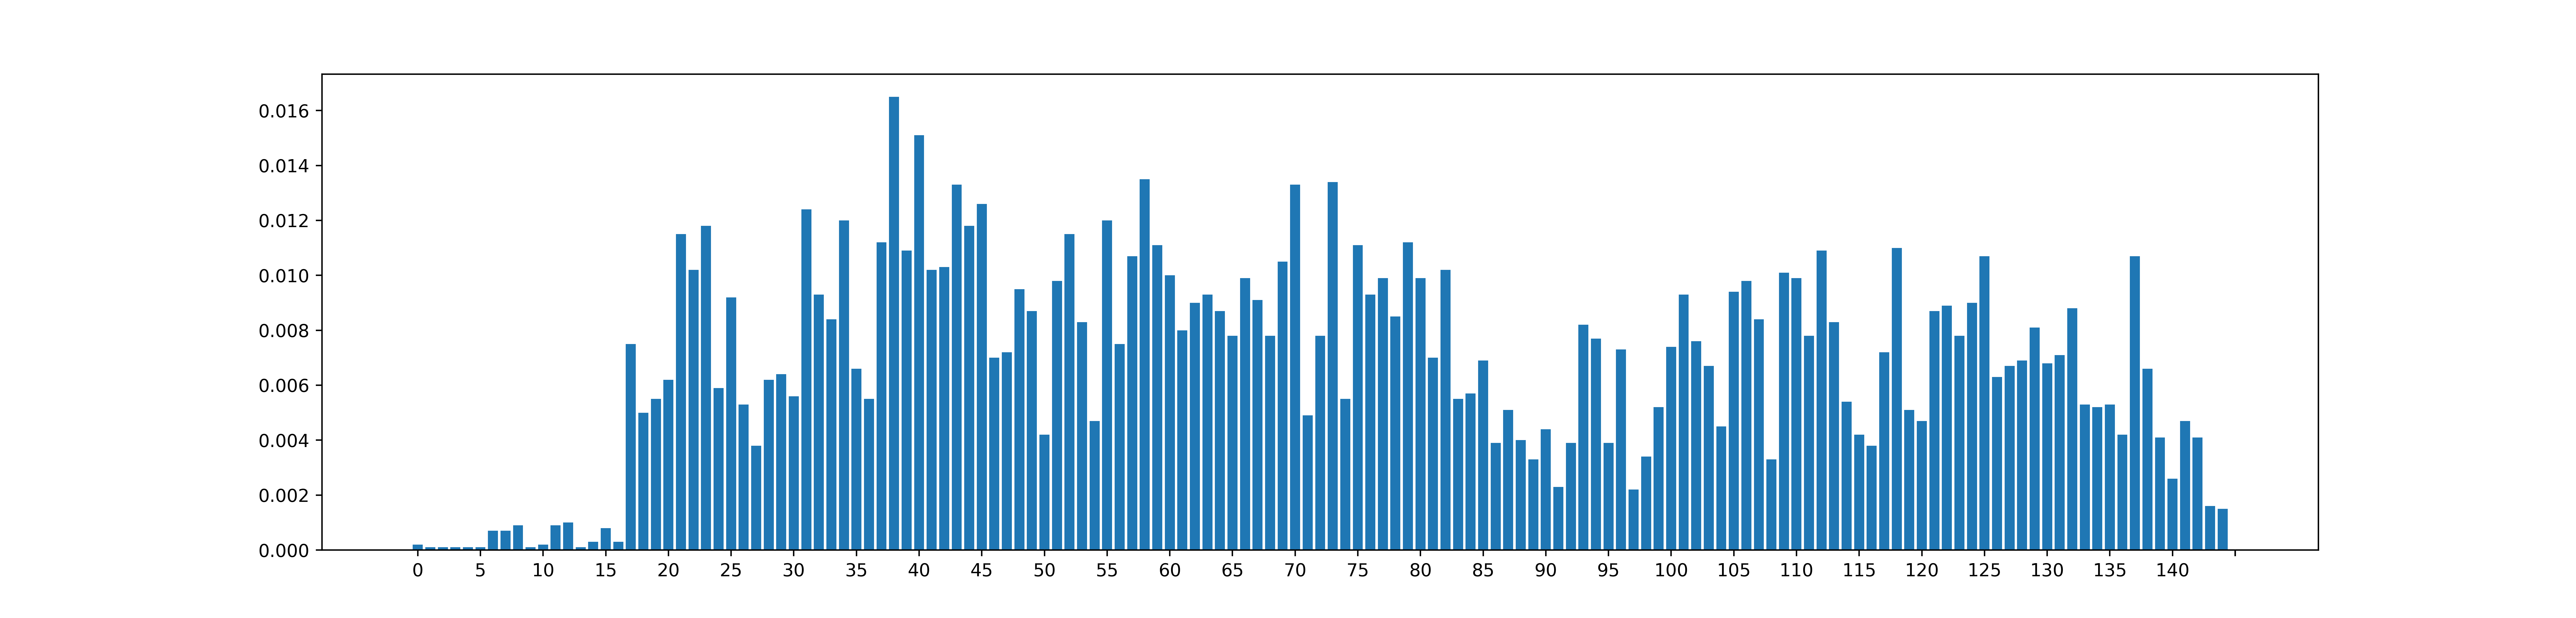
\includegraphics[trim={4cm 0cm 4cm 0cm}, clip, width=1\linewidth]{images/task 5.6.png}}
    \caption{Гістограма станів 4-розфарбовок}
    \label{figure: task 5.6}
\end{figure}

\begin{figure}[H]
    \center{\includegraphics[trim={4cm 4cm 4cm 4cm}, clip, width=1\linewidth]{images/task 5.5.png}}
    \caption{Графік $N=9$ ітерацій алгоритму МСМС}
    \label{figure: task 5.5}
\end{figure}

\newpage
\section*{Завдання 6}

\textit{За допомогою алгоритму вибірки Гіббса оцінити параметри ймовірності прокльовування яйця $p$ та кількості винесених куркою яєць $n$.} \\

Вибірка Гіббса -- різновид алгоритму МСМС для отримання вибірки із сумісного розподілу випадкових величин через почережний вибір з умовних розподілів: на кожному кроці одна змінна підправляється при фіксованих значеннях інших випадкових величин.

Тож при заданих параметрах $\lambda=10,\ a=b=1,\ x=7$, починаючи із наближення для кількості яєць $n=8$, алгоритм побудови вибірки Гіббса на $N=10\;000$ ланок матиме вид:

\begin{lstlisting}[firstnumber=1, label = code: task 6, caption = Генерування вибірки Гіббса]
    p, n = [], [8]
    for i in range(N):
        p.append(np.random.beta(x+a, n[-1]-x+b))
        n.append(x + np.random.poisson(lambda*(1-p[-1])))
\end{lstlisting}

\vspace{0.4cm}
В якості оцінки для параметра ймовірності прокльовування яйця $p$ візьмемо вибіркове середнє $\overline{p}:$
\[ \overline{p}=0.6856 \]  

Водночас, гістограми шуканих параметрів мають вид:

\begin{figure}[H]
    \begin{minipage}[H]{0.49\linewidth}
        \center{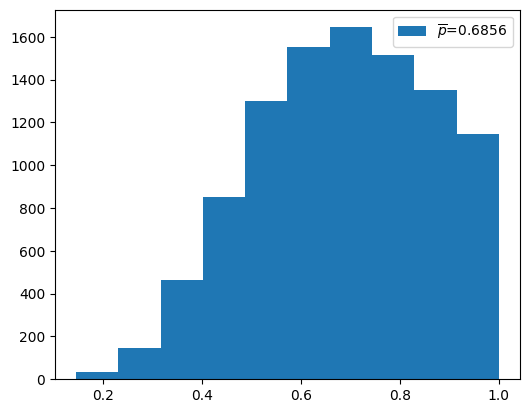
\includegraphics[width=1\linewidth]{images/task 6.1.png}} 
        а) Гістограма значень $p$
    \end{minipage}
    \hfill
    \begin{minipage}[H]{0.49\linewidth}
        \center{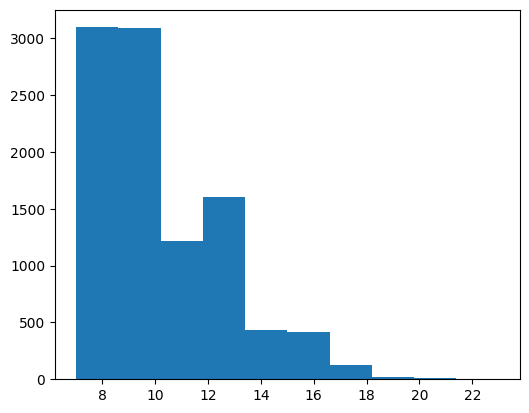
\includegraphics[width=1\linewidth]{images/task 6.2.png}} 
        б) Гістограма значень $n$
    \end{minipage}
\end{figure}

\newpage
\section*{Завдання 7}

\textit{Змоделювати заданий гаусовий розподіл як вибірку Гіббса.} \\

Розглянемо такий двовимірний гаусовий вектор:
\begin{equation*}
    \begin{psmallmatrix}
        x \\
        y \\
    \end{psmallmatrix}
    \sim N
    \left(
        \begin{psmallmatrix}
            0 \\
            0 \\
        \end{psmallmatrix}
        ,\;
        \begin{psmallmatrix}
            1 & \rho  \\
            \rho & 1 \\
        \end{psmallmatrix}
    \right),
\end{equation*}

де параметр коваріаційніної матриці покладемо $\rho=0.7$. Побудуємо такий ланцюг Маркова, для якого заданий розподіл є інваріантним. Тож починаючи з точки $(x_0,\;y_0)=(0.05,\;0.05)$, подальший алгоритм побудови ланцюга з $N=10\;000$ елементів виглядатиме так:

\begin{lstlisting}[firstnumber=1, label = code: task 7, caption = Генерування вибірки Гіббса]
    x0, y0 = 0.05, 0.05
    x, y = [x0], [y0]
    
    for i in range(N):
        x.append(np.random.normal(p*y[-1],1-p**2))
        y.append(np.random.normal(p*x[-1],1-p**2))
\end{lstlisting}

\vspace{0.4cm}
Зобразимо порівняльні тривимірні гістограми сумісних розподілів, тобто графіки частот потрапляння точок розподілу $(x,y)$ в певну числову область. Бачимо, що графiк вибірки, згенерованої засобами мови \texttt{Python}, доволі схожий з результатами генерації вибірки Гіббса:

\begin{figure}[H]
    \begin{minipage}[H]{0.49\linewidth}
        \center{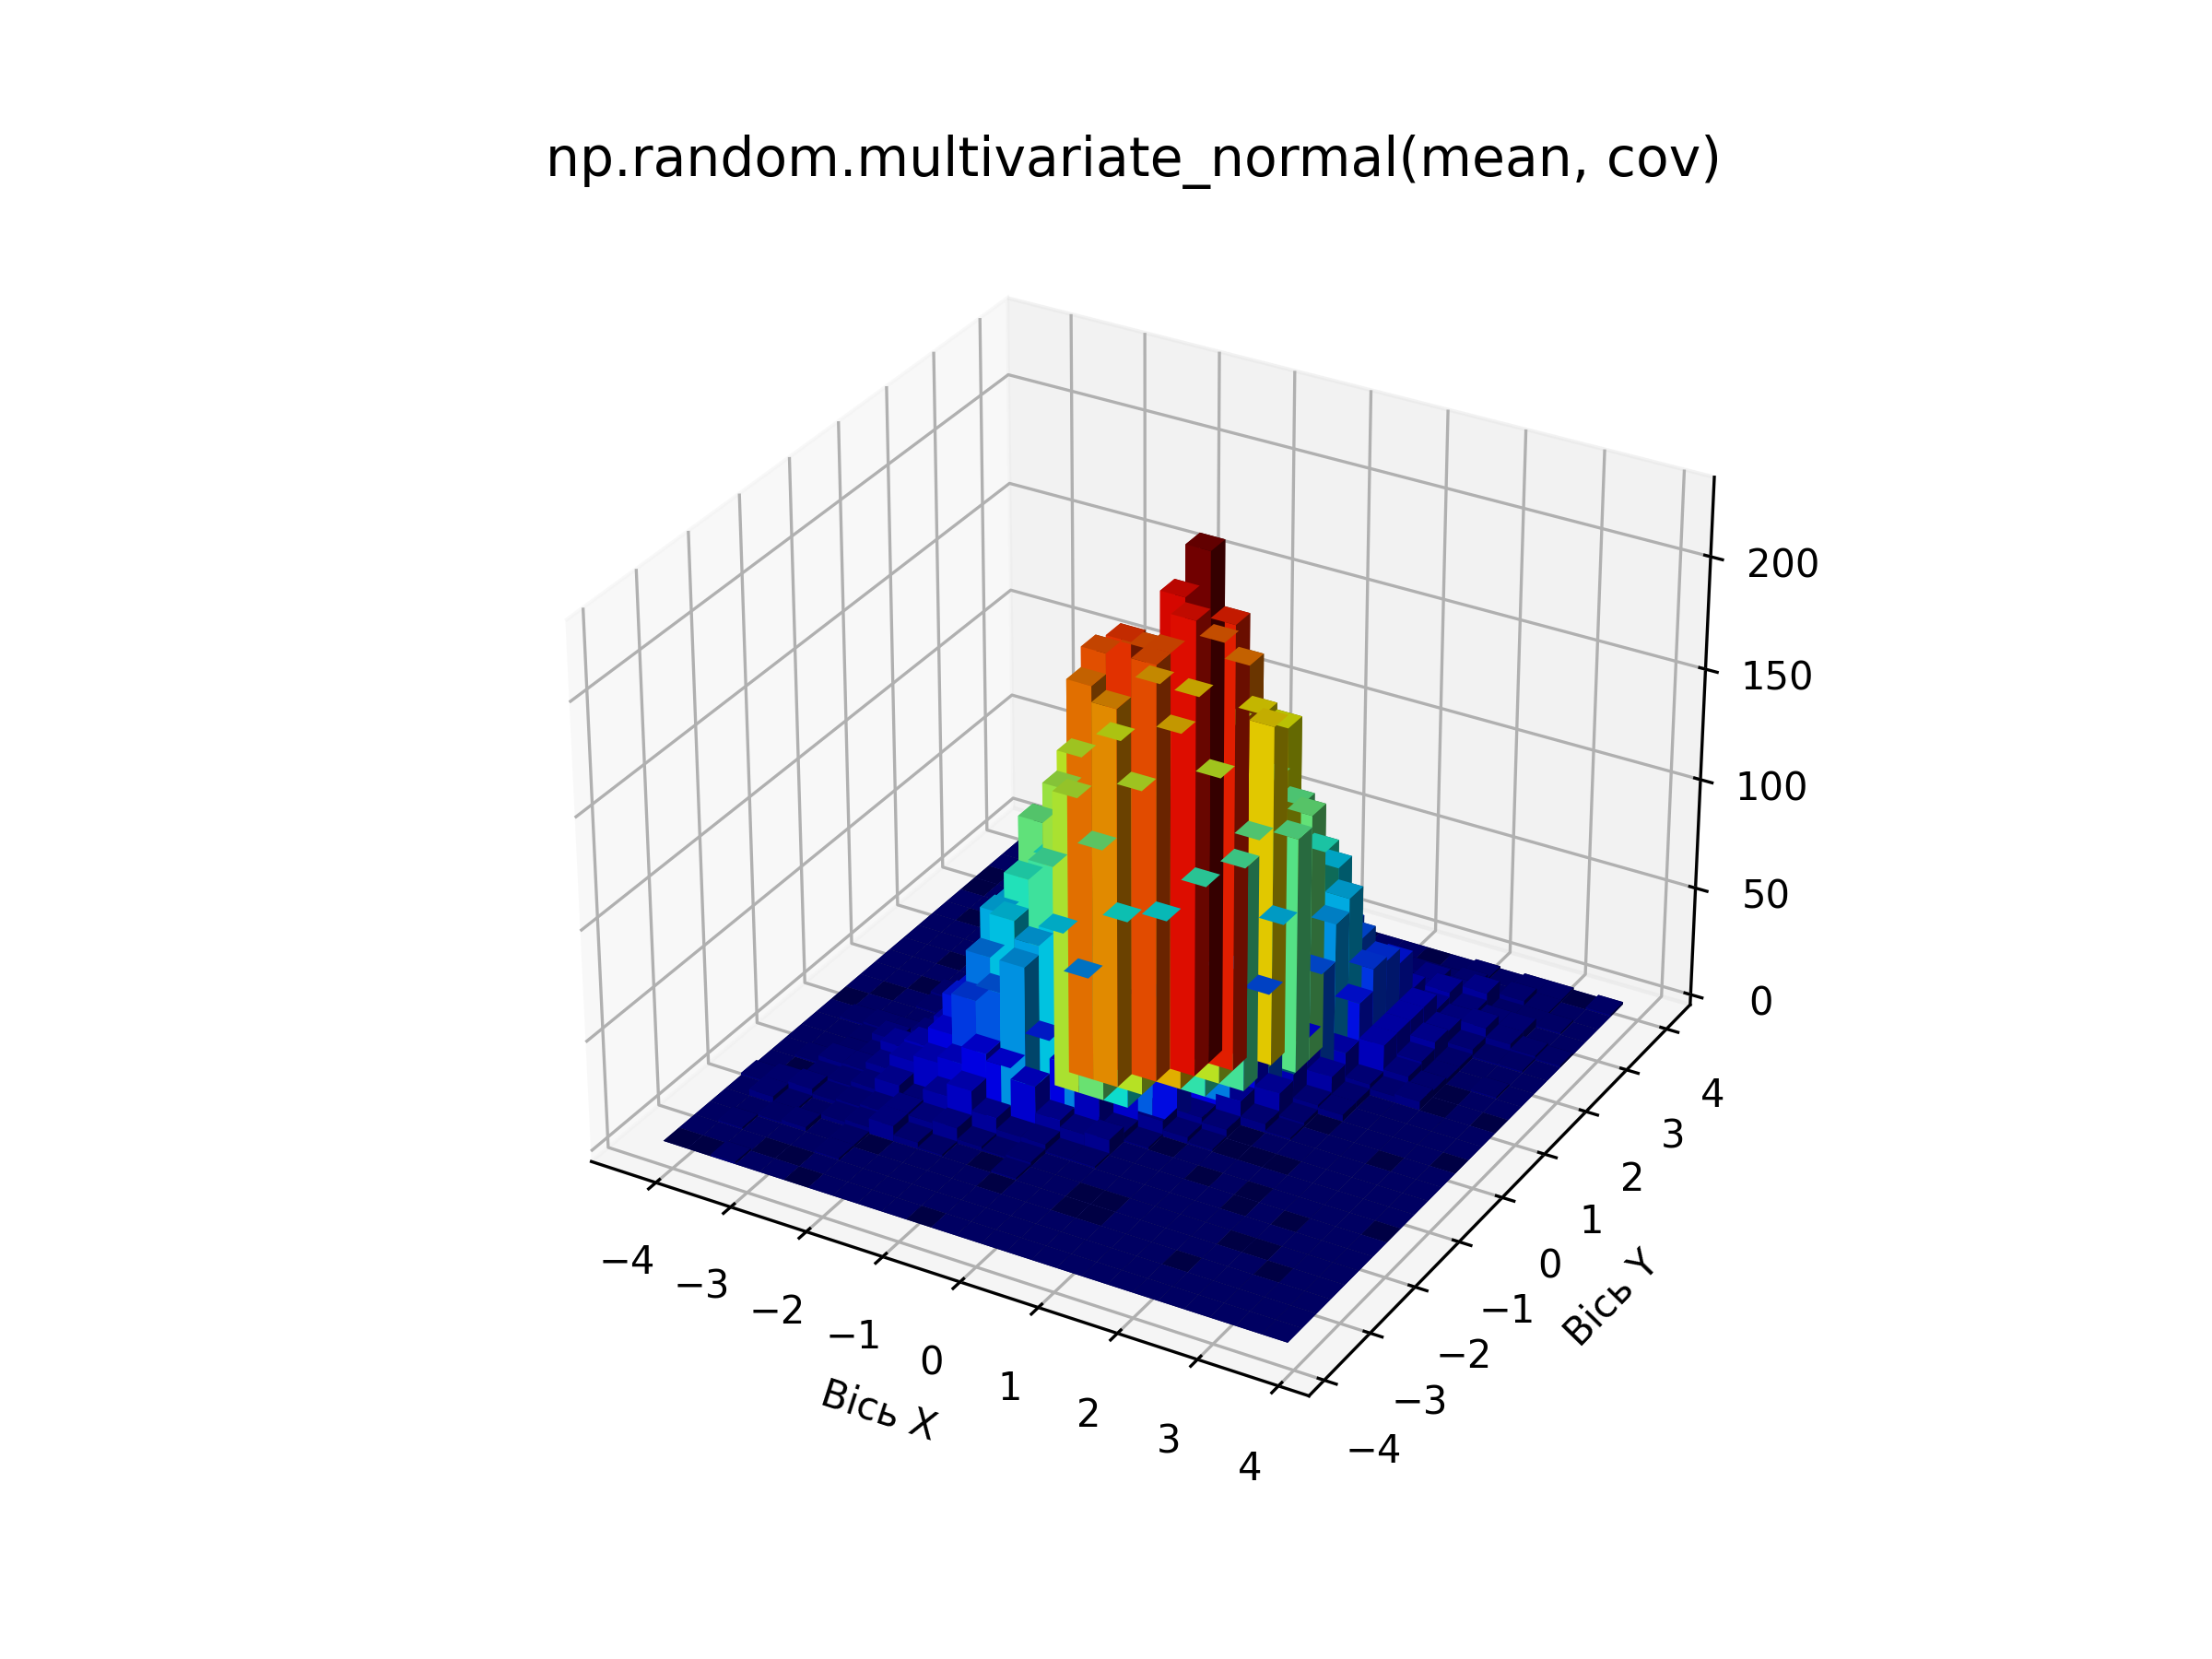
\includegraphics[trim={3cm 1.5cm 3cm 0сm}, clip, width=1\linewidth]{images/task 7.1.png}} 
        а) Генерація вбудованими методами мови \texttt{Python}
    \end{minipage}
    \hfill
    \begin{minipage}[H]{0.49\linewidth}
        \center{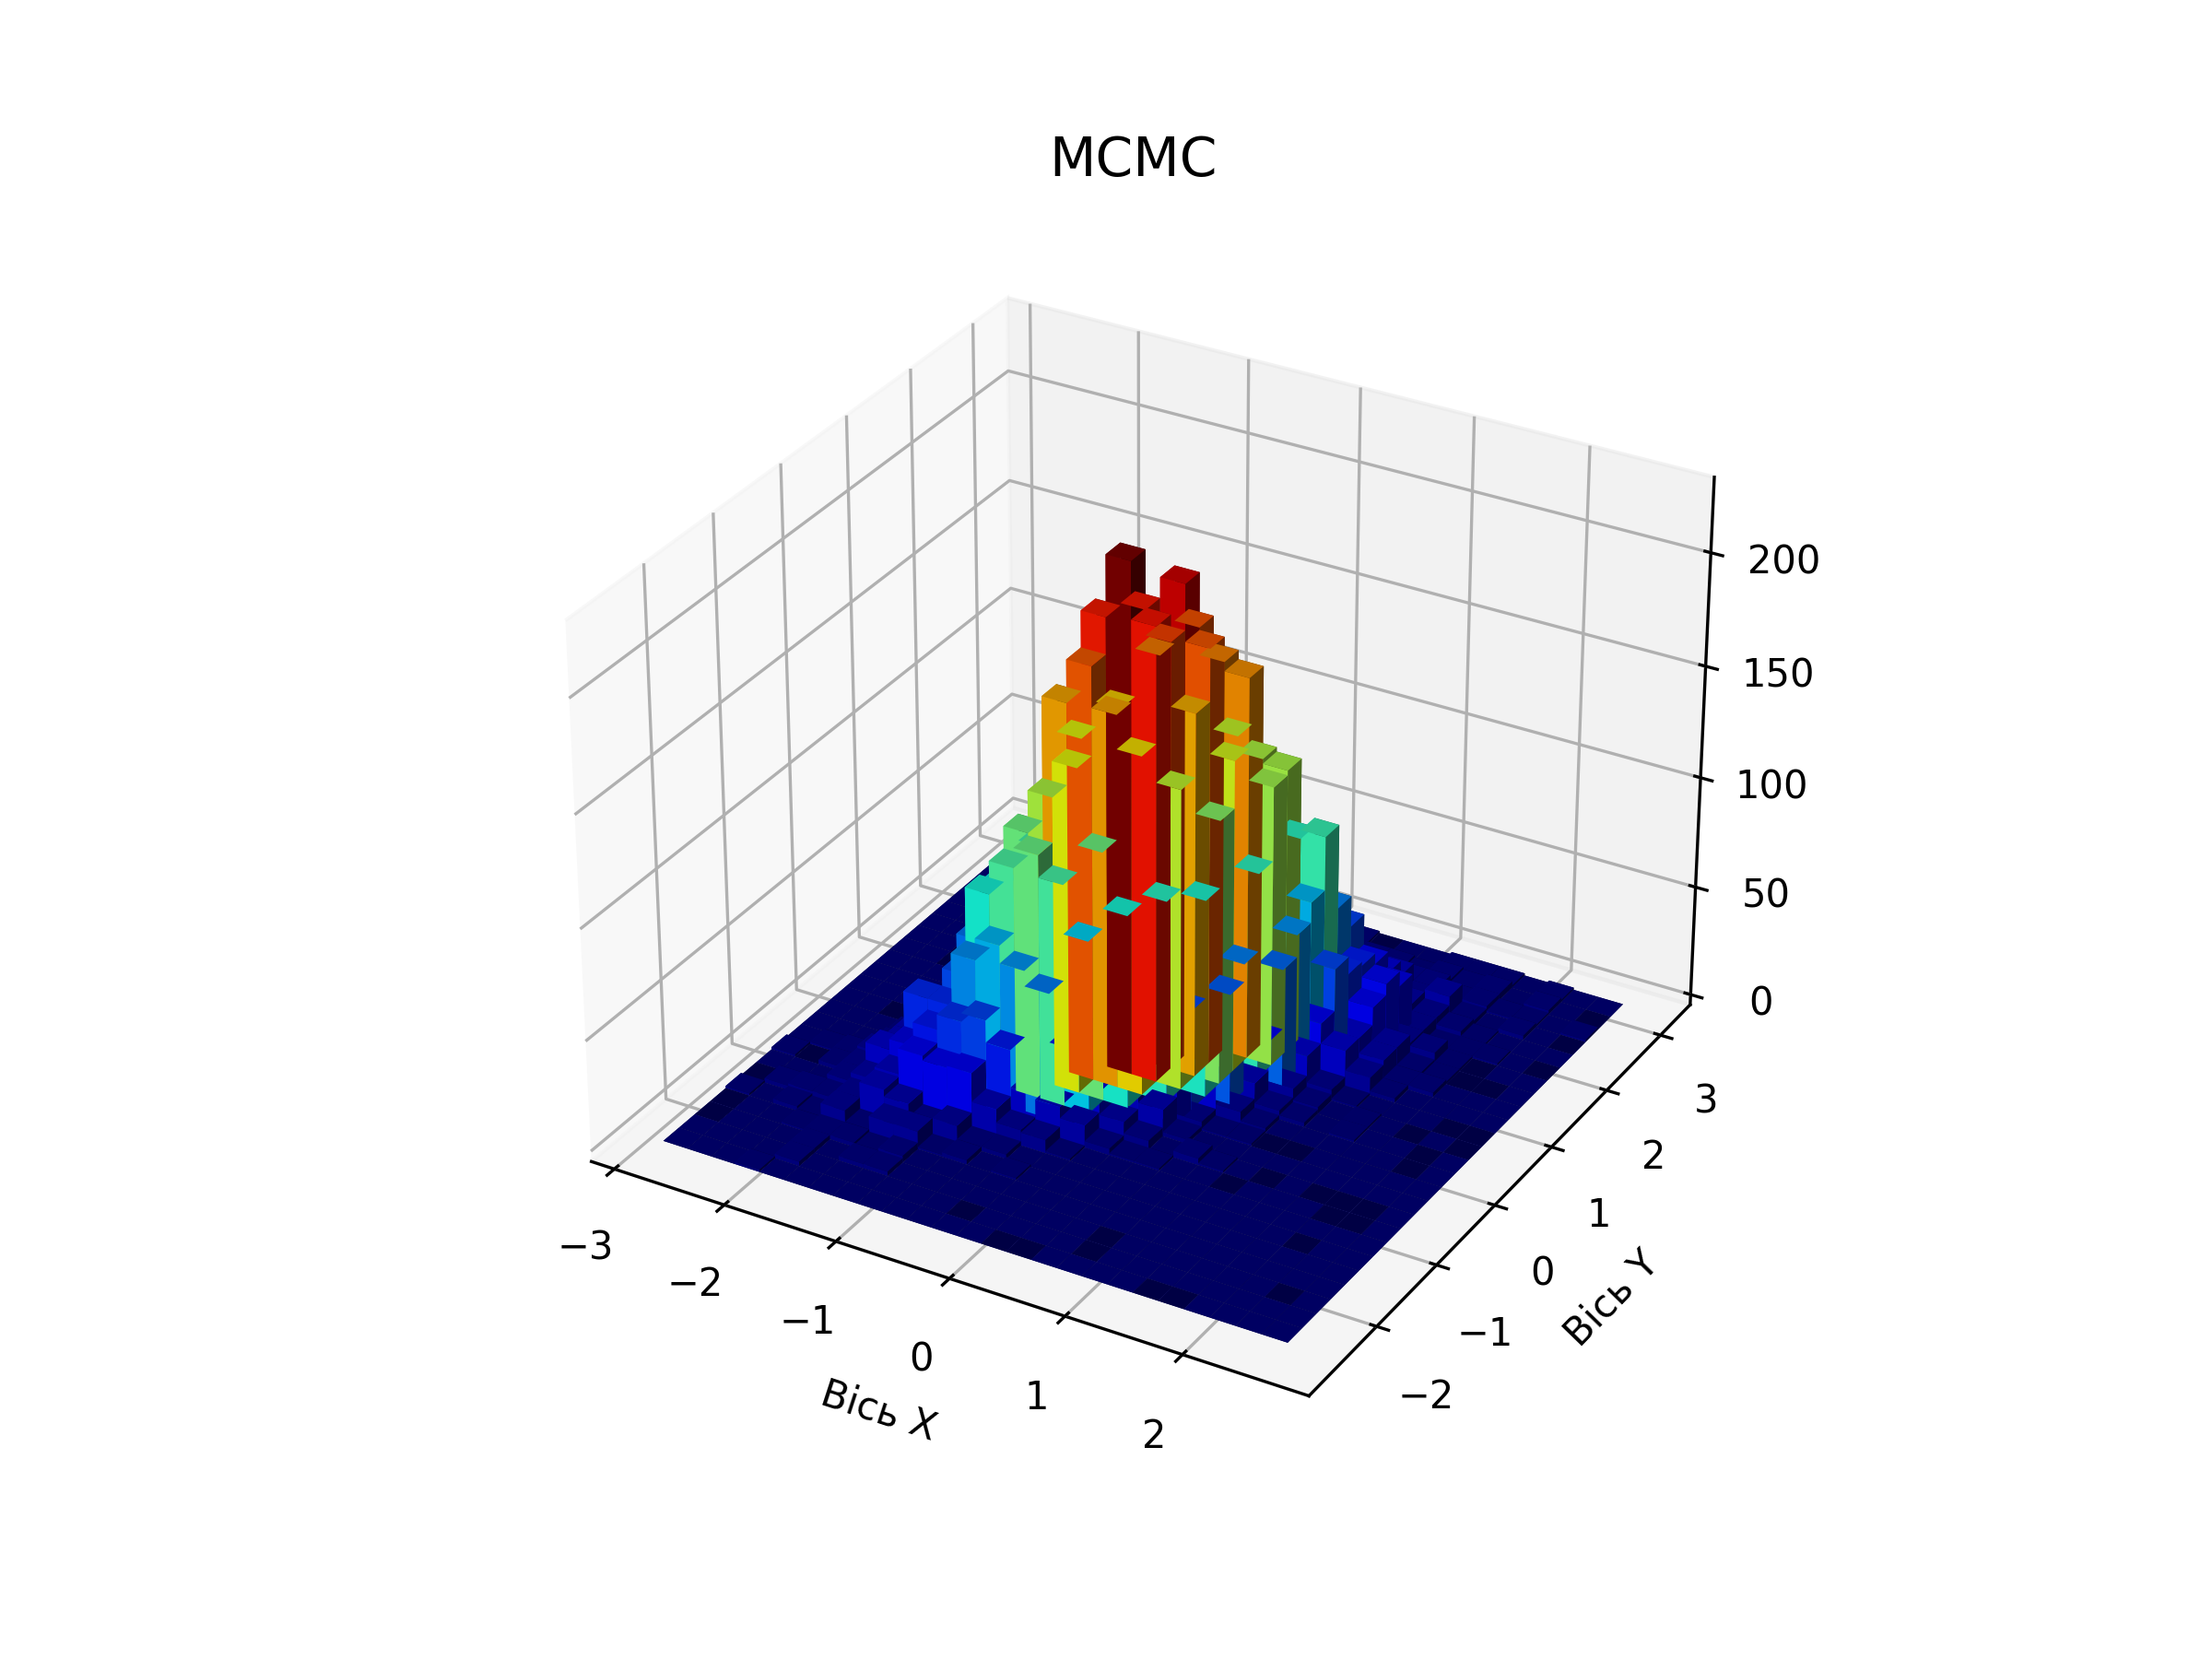
\includegraphics[trim={3cm 1.5cm 3cm 0cm}, clip, width=1\linewidth]{images/task 7.2.png}} 
        б) Генерація методами згідно умов Завдання 7
    \end{minipage}
\end{figure}

\newpage
\section*{Завдання 8}

\textit{За допомогою МСМС реалізувати випадкове блукання на множині таблиць спряженості ознак.} \\

Таблиця спряженості ознак $T$ -- це бінарна таблиця з фіксованим вектором $\overrightarrow{r}$ сум по стрічках та фіксованим вектором $\overrightarrow{c}$ сум по стовпцям. Позначимо множину $A(\overrightarrow{r},\overrightarrow{c})$ як множину всіх таких таблиць із заданими векторами $\overrightarrow{r}$ й $\overrightarrow{c}$.

Змоделюємо ланцюг Маркова на $A(\overrightarrow{r},\overrightarrow{c})$, де $\overrightarrow{r}=(3,2,1)$ й $\overrightarrow{c}=(2,2,1,1)$, так щоб інваріантний розподіл такого ланцюга збігався з рівномірним розподілом на $A(\overrightarrow{r},\overrightarrow{c})$. Еволюція таблиць спряженості в процесі генерування відбуватиметься через зміни так званих $[2\times 2]$ - шахматок -- пари стрічок та пари стовпців, на перетині яких стоїть матриця або 
$
    \begin{psmallmatrix}
        1 & 0 \\
        0 & 1 \\
    \end{psmallmatrix}
$, або
$
    \begin{psmallmatrix}
        0 & 1 \\
        1 & 0 \\
    \end{psmallmatrix}
$. 

Аналогічно до способу виявлення множини $k$-розфарбовок у Завданні 5, згенеруємо $N=10\;000$ ланок ланцюга, починаючи з таблиці
$
    \begin{psmallmatrix}
        1 & 1 & 1 & 0 \\
        1 & 1 & 0 & 0 \\
        0 & 0 & 0 & 1 \\
    \end{psmallmatrix}
$, й таким чином спробуємо оцінити кількість різних, унікальних таблиць спряженості ознак в множині $A(\overrightarrow{r},\overrightarrow{c})$.

Проте, перш ніж переходити до алгоритму МСМС, продемонструємо спосіб моделювання, за якого інваріантний розподіл утвореного ланцюга виявиться нерівномірним. Схематично такий алгоритм описано на Лістингу нижче:

\vspace{0.4cm}
\begin{lstlisting}[firstnumber=1, label = code: task 8.1, caption = Генерування ланцюга Маркова методом І (не МСМС)]
    T0 = [[1,1,1,0],
          [1,1,0,0],
          [0,0,0,1]]

    tables = [T0]
    
    for i in range(N):
        T = tables[-1]

        indexes = [k for k in range(len(T))]
        u = random.choice(indexes)
        indexes.remove(u)
        v = random.choice(indexes)

        indexes = [k for k in range(len(T[0]))]
        i = random.choice(indexes)
        indexes.remove(i)
        j = random.choice(indexes)

        current_checkerboard = [
            [T[min(u,v)][min(i,j)], T[min(u,v)][max(i,j)]],
            [T[max(u,v)][min(i,j)], T[max(u,v)][max(i,j)]]
        ]


        if current_checkerboard == [[1,0],[0,1]]:
            T[min(u,v)][min(i,j)], T[min(u,v)][max(i,j)] = 0,1
            T[max(u,v)][min(i,j)], T[max(u,v)][max(i,j)] = 1,0
            tables.append(T)

        elif current == [[0,1],[1,0]]:
            T[min(u,v)][min(i,j)], T[min(u,v)][max(i,j)] = 1,0
            T[max(u,v)][min(i,j)], T[max(u,v)][max(i,j)] = 0,1
            tables.append(T)
        
        else:
            tables.append(T)
\end{lstlisting}

\vspace{0.4cm}
Бачимо, що чергова таблиця може долучатися до ланцюга навіть якщо обрана $[2\times 2]$ - матриця не є шахматкою. Таким чином, за допомогою цього алгоритму виокремлено 8 різних станів серед елементів змодельованого ланцюга. Відстеження унікальних станів виконано аналогічним чином, як це описано в завданні генерування графів $k$-розфарбовок. Гістограма відвідин кожного з восьми станів зображена на Рис. \ref{figure: task 8.1}:

\vspace{0.4cm}
\begin{figure}[H]
    \center{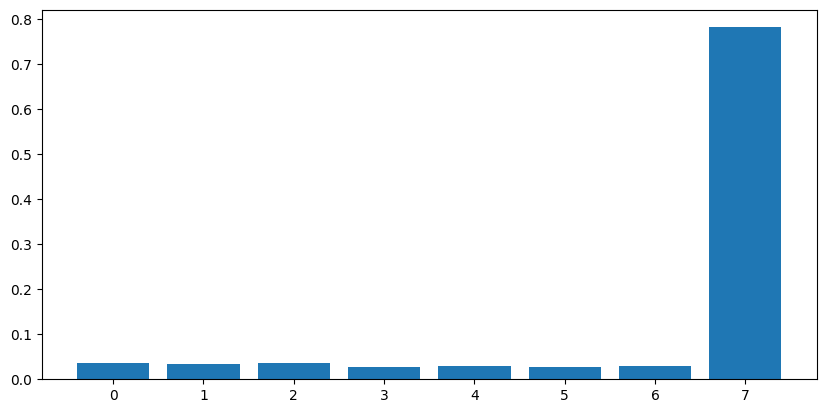
\includegraphics[width=0.9\linewidth]{images/task 8.1.png}}
    \caption{Гістограма згенерованого ланцюга за методом І (не МСМС)}
    \label{figure: task 8.1}
\end{figure}

Бачимо, що в стані <<7>>, який позначає таблицю $
\begin{psmallmatrix}
    1 & 1 & 0 & 1 \\
    1 & 1 & 0 & 0 \\
    0 & 0 & 1 & 0 \\
\end{psmallmatrix}
$, ланцюг проводить значну частину часу. Отже, попри те, що кількість різних станів ланцюга віднайдено коректно, інваріантний розподіл не є рівномірним.

У другому методі моделювання ланцюнга Маркова виникне потреба обчислення степені $d_i$ поточної таблиці $i$, тобто кількості $[2\times 2]$ - шахматок в $i$-тій таблиці спряжених ознак. Спосіб програматичного обчислення степені таблиці показано на Лістингу нижче. В силу великої кількості вкладених циклів \texttt{for loop} (а також в силу наявного в основному коді алгоритму циклу \texttt{while loop}) наведений раніше метод І (не МСМС) виявиться швидшим.

\begin{lstlisting}[firstnumber=1, caption = Функція визначення степені таблиці]
    def table_degree(T):
        checkerboard = [[[1,0],[0,1]], [[0,1],[1,0]]]

        d = 0
        for u in range(len(T)):
            for v in range(u+1,len(T)):
                for i in range(len(T[0])):
                    for j in range(i+1,len(T[0])):
                        current_checkerboard = [
                            [T[u][i], T[u][j]],
                            [T[v][i], T[v][j]]
                        ]

                        if current_checkerboard in checkerboard:
                            d += 1

        return d
\end{lstlisting}

\vspace{0.4cm}
Ймовірності $\alpha_{TT'}$ прийняття/відхилення для таблиці $T$ чергової пропозиції $T'$ матимуть вид:
\[ \alpha_{TT'}=\min\left\{ \frac{d_T}{d_{T'}}, \; 1 \right\},\]

де $d_T$ та $d_{T'}$ є степенями поточної та запропонованої таблиці відповідно. Отже, враховуючи усі введені позначення, схематично алгоритм генерування МСМС можна задати таким чином:

\begin{lstlisting}[firstnumber=1, label = code: task 8.2, caption = Генерування ланцюга Маркова методом ІІ (МСМС)]
    T0 = [[1,1,1,0],
          [1,1,0,0],
          [0,0,0,1]]

    tables = [T0]
    
    for i in range(N):
        T = tables[-1]

        while True:
            indexes = [k for k in range(len(T))]
            u = random.choice(indexes)
            indexes.remove(u)
            v = random.choice(indexes)

            indexes = [k for k in range(len(T[0]))]
            i = random.choice(indexes)
            indexes.remove(i)
            j = random.choice(indexes)

            current_checkerboard = [[T[min(u,v)][min(i,j)], T[min(u,v)][max(i,j)]],
                                       [T[max(u,v)][min(i,j)], T[max(u,v)][max(i,j)]]]

            if current_checkerboard in [[[0,1],[1,0]], [[1,0],[0,1]]]:
                break

        if current_checkerboard == [[1,0],[0,1]]:
            T[min(u,v)][min(i,j)], T[min(u,v)][max(i,j)] = 0,1
            T[max(u,v)][min(i,j)], T[max(u,v)][max(i,j)] = 1,0

            alpha = min(table_degree(tables[-1])/table_degree(T), 1)

            u = random.uniform(0,1)
            if u <= alpha:
                tables.append(T)
            else:
                tables.append(tables[-1])

        elif current_checkerboard == [[0,1],[1,0]]:
            T[min(u,v)][min(i,j)], T[min(u,v)][max(i,j)] = 1,0
            T[max(u,v)][min(i,j)], T[max(u,v)][max(i,j)] = 0,1
            
            alpha = min(table_degree(tables[-1])/table_degree(T), 1)

            u = random.uniform(0,1)
            if u <= alpha:
                tables.append(T)
            else:
                tables.append(tables[-1])

\end{lstlisting}

\vspace{0.4cm}
У такому разі згенерований ланцюг відвідуватиме 8 різних станів рівноміно, при чому кожна з компонент інваріантного розподілу буде мати достаньо близьке до $\frac{1}{8}$ значення:

\begin{figure}[H]
    \center{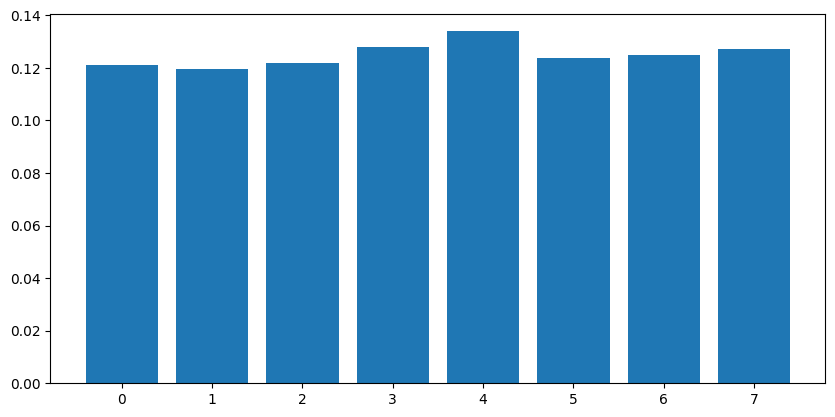
\includegraphics[width=0.9\linewidth]{images/task 8.2.png}}
    \caption{Гістограма згенерованого ланцюга за методом ІІ (МСМС)}
    \label{figure: task 8.2}
\end{figure}

\end{document} 